\tikzstyle{process} = [rectangle, rounded corners, minimum width=2cm, minimum height=1cm,text centered, draw=black, fill=gray!50]
\tikzstyle{decision} = [diamond, minimum width=2cm, minimum height=1cm, text centered, draw=black, fill=green!30]

% one line
%\begin{figure}[ht]
%    \centering
%    \begin{tikzpicture}[node distance=2cm]
%    %\draw[step=1cm,gray,very thin] (-8,-8) grid (8,8);
%	\node (Dataset) [process] {(Input) Nordjyske Dataset};
%	\node (Cleaning)[process, below of=Dataset] {(1) Preprocessing Phase};
%	\node (Training) [process, below of=Cleaning] {(2)Train IR Methods};
%	\node (Query) [process, below of=Training] {(3) Query Generation};
%	\node (Evaluate) [process, below of=Query] {(4) Evaluate Models};
%	\node (Result) [process, below of=Evaluate] {(Output) Results};
%	\draw [->, very thick] (Dataset) edge (Cleaning); 
%	\draw [->, very thick] (Cleaning) edge (Training);
%	\draw [->, very thick] (Training) edge (Query);
%	\draw [->, very thick] (Query) edge (Evaluate);
%	\draw [->, very thick] (Evaluate) edge (Result);
%\end{tikzpicture}
%	\caption{The method visualized as a flowchart, where a dataset consisting of articles is processed into a list of ranked results.}
%    \label{fig:process_figure}
%\end{figure}

\begin{figure}[ht]
	\centering
	\resizebox{\columnwidth}{!}{%
	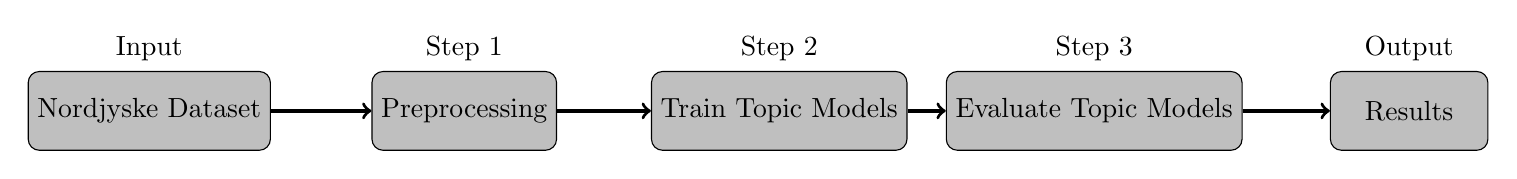
\begin{tikzpicture}[node distance=4cm]
	%\draw[step=1cm,gray,very thin] (-8,-8) grid (8,8);
	\node (Dataset) [process, label=above:{Input}] {Nordjyske Dataset};
	\node (Cleaning)[process, right of=Dataset, label=above:{Step 1}] {Preprocessing};
	\node (Training) [process, right of=Cleaning, label=above:{Step 2}] {Train Topic Models};
	\node (Evaluate) [process, right of=Training, label=above:{Step 3}] {Evaluate Topic Models};
	\node (Result) [process, right of=Evaluate, label=above:{Output}] {Results};
	\draw [->, very thick] (Dataset) edge (Cleaning); 
	\draw [->, very thick] (Cleaning) edge (Training);
	\draw[->, very thick] (Training) edge (Evaluate);
	\draw [->, very thick] (Evaluate) edge (Result);
	\end{tikzpicture}}
	\caption{The method visualized as a flowchart, where a dataset consisting of articles is processed into a list of evaluation results.}
	\label{fig:process_figure}
\end{figure}